\documentclass[sigconf, 9pt]{acmart}


\usepackage{xcolor}

\usepackage{float}
\usepackage{siunitx}


\newif\iffinal

% \finaltrue

\iffinal
  \newcommand{\tyler}[1]{}
  \newcommand{\ian}[1]{}
  \newcommand{\kyle}[1]{}
\else
  \newcommand{\tyler}[1]{{\textcolor{cyan}{ tyler: #1 }}}
  \newcommand{\ian}[1]{{\textcolor{red}{ Ian: #1 }}}
  \newcommand{\kyle}[1]{{\textcolor{purple}{ Kyle: #1 }}}
\fi


%%
%% \BibTeX command to typeset BibTeX logo in the docs
\AtBeginDocument{%
  \providecommand\BibTeX{{%
    \normalfont B\kern-0.5em{\scshape i\kern-0.25em b}\kern-0.8em\TeX}}}


\newcommand{\name}{Xtract}
\newcommand{\funcx}{$f$\kern-0.18em\emph{unc}\kern-0.05em X}

\acmConference{20th International Middleware Conference Doctoral Symposium}{2019}{Davis, CA}

\begin{document}


\title{Dredging a Data Lake: \\Decentralized Metadata Extraction at the Edge}

\author{Tyler J. Skluzacek} 
\affiliation{University of Chicago}
\email{skluzacek@uchicago.edu}


\renewcommand{\shortauthors}{Skluzacek et al.}

\begin{abstract}

The rapid generation of data from distributed IoT devices, scientific instruments, and compute clusters presents
unique data management challenges. The influx of large, heterogeneous, and complex data causes repositories to become 
siloed or generally unsearchable---both problems not currently well-addressed by distributed file systems.  
In this work, we propose \name{}, a serverless middleware 
to extract metadata from files spread across heterogeneous edge computing resources. 
In my future work, we intend to study how \name{} can
automatically construct file extraction workflows subject to 
users' cost, time, security, and compute allocation constraints. 
To this end, \name{} will enable the creation of a searchable centralized index across distributed data collections.


\end{abstract}

\begin{CCSXML}
<ccs2012>
<concept>
<concept_id>10002951.10003227.10010926</concept_id>
<concept_desc>Information systems~Computing platforms</concept_desc>
<concept_significance>500</concept_significance>
</concept>
<concept>
<concept_id>10002951.10003317.10003365.10003366</concept_id>
<concept_desc>Information systems~Search engine indexing</concept_desc>
<concept_significance>300</concept_significance>
</concept>
<concept>
<concept_id>10010405.10010497.10010500.10010503</concept_id>
<concept_desc>Applied computing~Document metadata</concept_desc>
<concept_significance>500</concept_significance>
</concept>
</ccs2012>
\end{CCSXML}

\ccsdesc[500]{Information systems~Computing platforms}
\ccsdesc[500]{Applied computing~Document metadata}
\ccsdesc[300]{Information systems~Search engine indexing}

\keywords{data lakes, serverless, metadata extraction, file systems}

\maketitle


\section{Introduction}

The rapid generation of data from IoT devices, scientific instruments, simulations, and myriad other sources presents unique 
data management challenges. Currently data are stored across multiple machines, are often siloed, and require 
significant manual labor to create metadata that promote usability and searchability. 
Some~\cite{egan2003vizier, dataverse}  have created data catalogs from user-submitted metadata. These, however, are not scalable to current and future storage systems,
as humans cannot possibly label billions of heterogeneous files.   
In order to better organize, discover, and act upon distributed big data, 
we first require automated methods to crawl file systems and extract 
metadata for each file therein. 
While others have developed end-to-end automated metadata extraction systems, 
they require that data be moved to a central service~\cite{skluzacek2018skluma, skluzacek2016klimatic, padhy2015brown, rodrigo2018sciencesearch} or lack built-in scaling capabilities~\cite{mattmann2011tika}. 
In this work we strive to create a flexible, scalable, and decentralized metadata extraction system that 
can be employed centrally or at the edge. 

We present our prototype and vision for \name{},
a decentralized middleware that provides high-throughput and on-demand metadata 
extraction, enabling the automated creation of rich, searchable data lakes from unsearchable data silos. 
We leverage a Function as a service (FaaS) model for managing the invocation of
many short-running extractors on an arbitrarily large number of files. 
The current \name{} implementation uses the \funcx{} serverless supercomputing platform~\cite{chard2019serverless}
to execute functions across diverse and distributed computing infrastructure.  
The advantage of using \funcx{} is that it allows us to explore a novel distributed FaaS model 
that overcomes the need to move large amounts of data to the cloud. 
Instead, \name{} is able to push
metadata extractors to the edge systems on which the scientific data reside. 
We envision that \name{} could also use other edge computing fabrics, 
such as Amazon Web Services IoT Greengrass or Google Cloud IoT. 
The primary contributions of \name{} are: 
\begin{itemize}
\item Scalable across distributed computing resources, including laptops, clusters, and edge devices.
% IoT to HPC, and across multiple edge computing fabrics. 
\item Flexible extraction model that can be deployed centrally or at the edge, facilitating decentralized metadata extraction.
\item Supports dynamic construction of customized extractor pipelines for diverse file types. 
\item Intelligently executes data staging decisions based on user-supplied constraints, including time, cost, compute allocation availability, and security. 
%\item Automatically populates a search index of rich metadata. 
\end{itemize}


\section{Approach}
\label{sec:approach}

\name{} is a decentralized middleware that provides for distributed metadata extraction. 
The \name{} service plans dynamic metadata extraction pipelines, comprised of specialized
metadata extractor functions, and coordinates the execution of those extractors
either locally or at the edge, subject to various constraints. 
%, including extraction time, cost, available compute allocations, and security policies. 
An example two-site deployment of \name{} is shown in Figure~\ref{fig:arch}. 
The remainder of this section 
details \name{}'s core components and design goals.

\textbf{Metadata extractors} are functions that input a file or group of files, and output a metadata dictionary. 
Each metadata extractor runs in a given container runtime with all required dependencies (i.e., files and 
libraries).  \name{} currently provides a number of built-in extractors, including
those to identify null values in tabular files, nesting patterns in structured XML files, topics and keywords from free text, and location tags from map images, 
among others~\cite{skluzacek2019serverless}. In future work, 
we plan to support user-submitted metadata extractors, automatically generate (and potentially share) runtime containers based on inferred 
dependency requirements, and train \name{} to recognize when it is appropriate to apply user-submitted extractors in each file's metadata extraction workflow. 

The \textbf{\name{} service} dynamically applies a set of metadata extractors to each file in the repository. 
First, \name{} sends a crawler function to the data and populates a metadata dictionary for each file containing
its filesystem properties (e.g., path, size, extension).  Once the initial dictionary is created, \name{} invokes a file type extractor on each 
file that is used to select downstream extractors. We have shown that feeding 
the first $n$ bytes of a file as features into 
a trained model can predict the appropriate first extractor functions to apply to a file, in significantly less time
than attempting to execute incorrect extractors on each file~\cite{skluzacek2018skluma}. Once this first extractor function returns metadata, the \name{} service dynamically selects additional extractors to apply based on the output.  For instance, 
a tabular file with a multi-line free text header (e.g., describing experimental setup) is identified by \name{} as first requiring a tabular extractor, but 
the resultant metadata will denote free text parts of the file that can benefit from keyword and topic extractors.
\name{} protects requests to the web service using Globus Auth~\cite{tuecke2016globus}, and stores metadata to a Globus Search index. 

\textbf{Endpoints} are the edge computing fabric that provision compute resources and execute functions in container runtimes for files on the local file system.
 Endpoints can currently be deployed across myriad compute providers such as IoT devices, cloud instances, and clusters.  
Endpoints deployed in \funcx{} utilize the Parsl~\cite{babuji2019parsl} parallel programming library to 
provision compute resources, and to manage the execution of functions in containers on provisioned resources. Endpoints enable 
\name{} to execute metadata extraction functions at any registered and accessible endpoint. 
We have shown that deploying \funcx{} 
endpoints on HPC systems allows \name{} to reliably
scale to deploy millions of metadata extraction functions 
across thousands of nodes spanning multiple compute locations~\cite{chard2019serverless}. 


\begin{figure}[t]
	\centering
	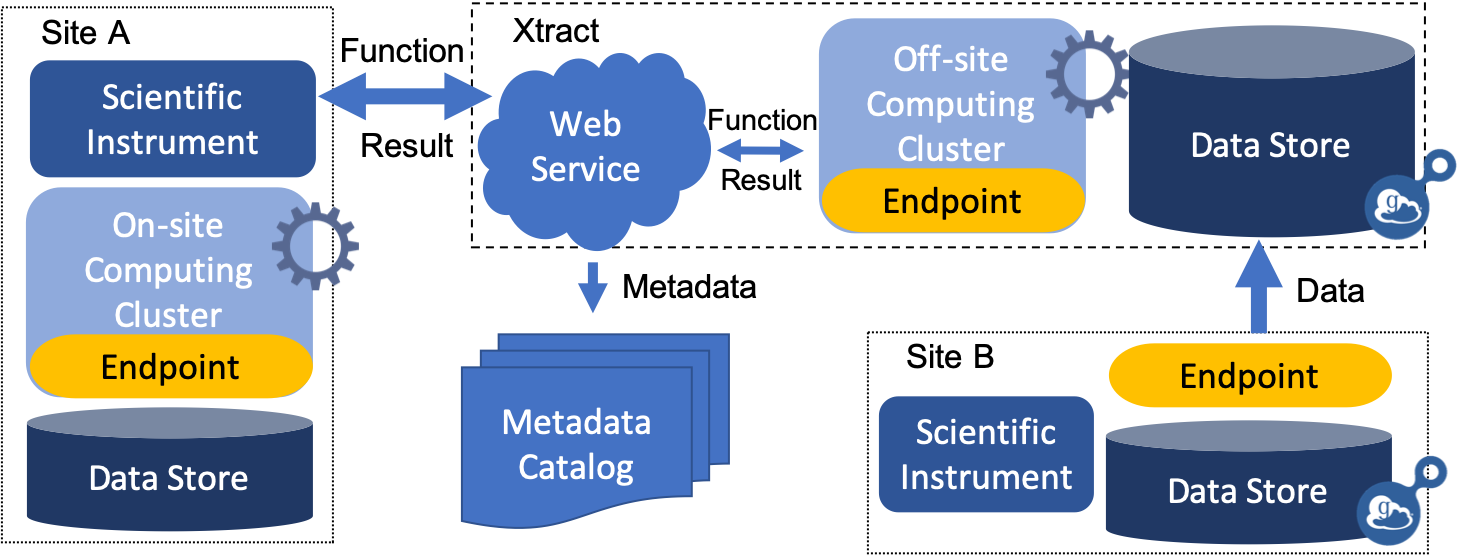
\includegraphics[scale=0.17]{figs/updated-fig.png}
	\caption{Overview of the \name{} architecture. For \textit{Site A} extractors are transmitted to the remote resource for execution on local computing resources, returning metadata to the \name{} service. 
    \textit{Site B} lacks suitable local computing capabilities, requiring data to be staged to \name{} for extraction.}
	\label{fig:arch}
\end{figure}


\section{Evaluation Plan}
\label{sec:eval}

In future work we plan to study how \name{} can self-optimize subject to real-world, user-defined constraints for heterogeneous data stored across multiple 
endpoints.  Specifically, we plan to explore how augmenting metadata extraction workflows to stage data to idle or under-utilized resources could 
find globally optimal extraction strategies with respect to diverse user constraints of financial cost, computing time, security, and compute resource allocation 
availability or volatility.

We intend to evaluate \name{}'s self-optimization strategies subject to a large number of constraint combinations across a diversity of datasets. 
These include the Carbon Dioxide Information Analysis Center (330+ GB, 10,000+ 
unique file extensions of carbon dioxide data), the Materials Data Facility~\cite{ blaiszik2019mdf} (30+ TB, tens of millions of materials science files); 
Petrel (4+ PB, 50,000+ files of cross-disciplinary data at Argonne National Lab), and Globus (20,000+ unique, connected 
endpoints containing hundreds of billions of files).


\section{Conclusion}
\label{sec:conc}

\name{} enables users to search and organize large, distributed data sets by employing dynamic metadata extraction workflows to construct a rich index over all files in the set.
\name{} is a middleware that addresses data locality and scalability challenges by deploying compute endpoints on the edge
devices and constructing these workflows subject to a number of user constraints. Such a system will enable researchers, companies, and individuals alike to more easily find, understand, and share increasingly 
complex data sets, leading to enhanced scientific and industrial progress. 


\begin{acks}

This research is conducted under the guidance of Dr. Ian Foster and Dr. Kyle Chard, and with contributions
from Dr. Ryan Chard, Dr. Zhuozhao Li, Yadu Babuji, and Ryan Wong. We gratefully acknowledge the use of compute 
resources from the Jetstream cloud for science and engineering~\cite{jetstream}.


\end{acks}
\bibliographystyle{ACM-Reference-Format}
\bibliography{wosc}


\end{document}
\endinput
